\documentclass[11pt]{article}
\usepackage{verbatim}
\usepackage{listings}
\usepackage{array}
\usepackage{xcolor}
\usepackage{graphicx}
\graphicspath{{.}}

\usepackage{blindtext}
\usepackage{hyperref}
\hypersetup{
    colorlinks=true,
    linkcolor=blue,
    filecolor=magenta,      
    urlcolor=cyan,
    pdftitle={Overleaf Example},
    pdfpagemode=FullScreen,
    }

\definecolor{codegreen}{rgb}{0,0.6,0}
\definecolor{codegray}{rgb}{0.5,0.5,0.5}
\definecolor{codepurple}{rgb}{0.58,0,0.82}
\definecolor{backcolour}{rgb}{0.93,0.95,0.95}

\lstdefinestyle{nabla}{
    backgroundcolor=\color{backcolour},   
    commentstyle=\color{codegreen},
    keywordstyle=\color{magenta},
    numberstyle=\tiny\color{codegray},
    stringstyle=\color{codepurple},
    basicstyle=\ttfamily\footnotesize,
    breakatwhitespace=false,         
    breaklines=false,                 
    captionpos=b,                    
    keepspaces=true,                 
    numbers=left,                    
    numbersep=5pt,                  
    showspaces=false,                
    showstringspaces=false,
    showtabs=false,                  
    tabsize=2
}
\lstset{style=nabla}

\title{Datenraffinerie Manual}
\author{Alexander Becker}
\date{\today}

\begin{document}
\maketitle
\tableofcontents
\pagebreak
\section{Introduction and Overview}
\subsection{Motivation}
As HGCAL moves from a few prototype boards and modules to preproduction seeing dozens of modules and test systems in use throughout the collaboration a coherent software environment is increasingly needed on the one hand to reduce the confusion caused by multiple different processes to acquire data from the different test systems and on the other hand reduce the duplicate effort by different groups of the collaboration by having a common set of tools and procedures.

The Datenraffinerie is the Attempt to create a coherent and user friendly way to acquire characterization and beam-test data from the Hexaboard using a Hexacontroller (a.k.a the test system). The Datenraffinerie is a set of command line tools and services that together acquire raw data from the Hexaboard or module and process it so that it can be easily analysed using the \texttt{python} and the many utilities that the \texttt{pandas} package provides.

\section{Overview}
The Datenraffinerie consists of two groups of programs. There are the Services that need to be run on the Hexacontroller and another computer called the \emph{Coordinator}. The second group of programs are the command line tools that the user primarily interacts with, that are run on the \emph{Client} which is also where the raw data is delivered too.

\subsection{Services}
\begin{figure}
	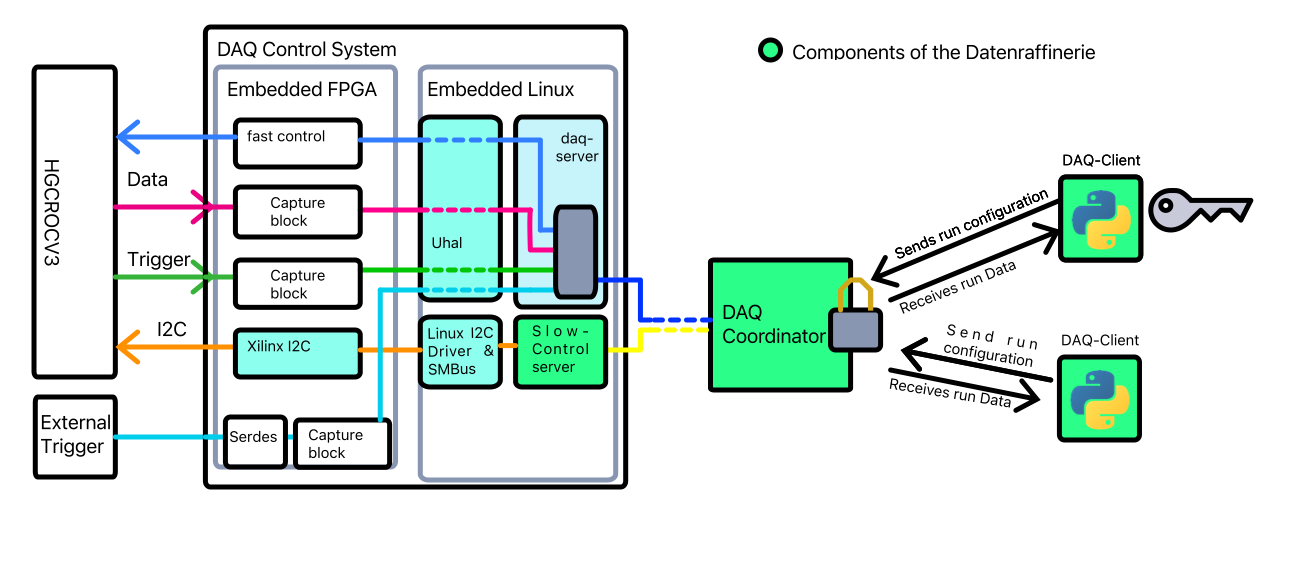
\includegraphics[width=\textwidth]{datenraffinerie-daq-setup}
	\label{fig:overview}
\end{figure}
There are a total of three services that are part of the Datenraffinerie
\begin{itemize}
	\item \texttt{daq-server}: Acquires Data from the ROCs and builds the fast-command stream
	\item \texttt{sc-server} : Configures and reads out the parameters of the ROCs
	\item \texttt{daq-coordinator} : Coordinates access to the Hexacontroller between different clients
\end{itemize}
The \texttt{sc-server} and \texttt{daq-server} are both run on the Hexacontroller. The \texttt{daq-server} is in charge of generating a fast command stream for the ROCs on the Hexaboard and collecting the resulting Trigger and DAQ Streams. Due to the limited resources on the Hexacontroller 

The \texttt{sc-server} or \emph{slow-control-server} is in charge of configuring the HGCROCs on the Hexaboard according to the specifications of the measurement. It connects to the HGCROCs via the I$^2$C protocol and can read and write all the parameters to and from the chip.

The last of the services is the \emph{DAQ-coordinator}. It controls the access to the Hexacontroller so that no two clients can write commands to the Hexacontroler simultaneously and thus invalidating the data. The DAQ-Coordinator also provides some simplification on the side of the message interface.

Besides these services, the Datenraffinerie relies on the \texttt{daq-server} that is part of the \texttt{hexactrl-sw} git repository. The software can be found \href{https://gitlab.cern.ch/hgcal-daq-sw/hexactrl-sw}{on the CERN gitlab}. As displayed in

\subsection{Command Line Tools}
There are three command line tools that make up the core of the user facing part of the Datenraffinerie.
\begin{itemize}
	\item \texttt{generate-configs}
	\item \texttt{acquire-data}
	\item 	\texttt{process-raw-data}
\end{itemize}

The \texttt{generate-configs} program generates a directory containing all informations that is needed for the procedure. The name is user selectable and will be called \texttt{procdir} for the remainder of this manual. It reads in the datenraffinerie configuration files and then produces all necessary files from that, which it places into \texttt{procdir}.

The \texttt{acquire-data} program uses the information contained in the folder produced by the \texttt{generate-configs} to perform the data acquisition. It places the acquired data into the \texttt{procdir}.

The \texttt{process-raw-data} command converts the data produced acquired by the \texttt{acquire-data} command into \texttt{*.h5} files that contain columns both from the acquired data and from the configuration of the chip. The \texttt{*.h5} files can be loaded into pandas \texttt{DataFrames} for analysis and can be configured to contain all information necessary for analysis. 

\subsection{Additional tools}
There are two more command line tools that help the user make sense of the configuration and State of the ROCs. These are
\begin{itemize}
	\item \texttt{read-rocs}
	\item \texttt{yaml-utils}
	\item \texttt{show-hdf}
\end{itemize}  
The \texttt{read-rocs} command connects directly to the \texttt{sc-server} without talking to the daq-coordinator first. It can be used to read, reset and configure the ROCs directly. It uses the same interface as the \texttt{daq-coordinator} and is intended to be used during debugging of procedures.

The \texttt{yaml-utils} command line tool can be used to update and compare different yaml files. It uses the same comparison and merging functions as the Datenraffinerie and is intended to help make sense of the different configurations during debugging of a procedure.

The \texttt{show-hdf} tool prints a section of the \texttt{hdf} file produced by the \texttt{process-raw-data} command and is useful to quickly check the properties of the output files.
\subsection{C++ Utilities}
To be able to handle the large amounts of data that can be produced by a single run of a procedure, the transformation from `raw` data to the \texttt{*.h5} files is performed by custom commands that are compiled from C++ code. This makes the transformation up to 200 times faster compared with an implementation in python.
The \texttt{fracker} tool merges the data acquired by the Datenraffinerie with the configuration of the chip to produce a single \texttt{*.h5} file containing both the configuration of the system and the data gathered during the run.

The \texttt{turbo-pump} is able to concatenate multiple files of the same run into the same \texttt{h5} file. With the version 1 of the Datenraffinerie it has fallen into disuse, although it makes it possible to combine smaller files produced by the runs of the same procedure into a single file, making analysis simpler by eliminating the need to combine the results of a partial analysis running on every one of the files.

The C++ tools are run by the Datenraffinerie command line tools and the user will neither need to manually run the \texttt{fracker} nor the \texttt{turbo-pump}.

To install these tools a set of steps need to be performed that are separate from the steps needed to be taken to install the python part of the Datenraffinerie.

\subsection{External Software}
Currently the Datenraffinerie relies on the \href{https://gitlab.cern.ch/hgcal-daq-sw/hexactrl-sw}{hexactrl-sw} for various parts of the system. As mentioned before, the \texttt{daq-server} needs to be installed on the hexacontroller, and the \texttt{daq-client} needs to be installed on the computer running the \texttt{daq-coordinator}. The \texttt{daq-server} can be installed on the hexacontrollers via an RPM package.

The Datenraffinerie expects the \texttt{daq-client} to be in the \texttt{\$PATH}, which needs some manual linking if the client side software is also installed via the RPM package. For more information please contact Arnaud Steen.

\section{Installation}
To install the Datenraffinerie, the \texttt{daq-client} needs to be installed on the computer running the \texttt{daq-coordinator}. No other C++ tools are needed on this machine. Along with the \texttt{daq-client} the python part of the Datenraffinerie needs to be installed.

On the \emph{client} the C++ tools of the Datenraffinerie, the \texttt{fracker} and \texttt{turbo-pump} need to be installed along with the python part of the Datenraffinerie.
\subsection{Prerequisites}
It is recommended that the \emph{coordinator} and the \emph{client} be desktop-like computers running at least CentOS-8. For installation instructions on the \texttt{daq-client} please contact Arnaud Steen for further assistance. To install the C++ tools of the Datenraffinerie the following packages need to be installed on the CentOS-8 client computer:
\begin{itemize}
	\item \texttt{cmake}
	\item \texttt{glibc}
	\item \texttt{hdf5}
	\item \texttt{libaec}
	\item \texttt{libgcc}
	\item \texttt{libstdc++}
	\item \texttt{libzstd}
	\item \texttt{lz4-libs}
	\item \texttt{openssl-libs}
	\item \texttt{pcre}
	\item \texttt{root-core}
	\item \texttt{root-io}
	\item \texttt{root-mathcore}
	\item \texttt{root-multiproc}
	\item \texttt{root-net}
	\item \texttt{root-ttree}
	\item \texttt{tbb}
	\item \texttt{xxhash-libs}
	\item \texttt{xz-libs}
	\item \texttt{yaml-cpp}
	\item \texttt{zlib}
	\item \texttt{python3.9}
\end{itemize}
Even though these packages may be available on CentOS 7 the versions of the software in the packages are not sufficient to build the C++ tools of the Datenraffinerie. Therefore it is \emph{necessary} to at least run CentOS 8.

The with these packages installed the datenraffinerie can be cloned from \texttt{https://gitlab.cern.ch/hgcal-daq-sw/datenraffinerie} into a directory of the users choice.

The current source code of the Datenraffinerie is located on the \texttt{dev} branch of the Repository.

\subsection{Installing the C++ Tools}
The source code for the C++ tools can be found in the \texttt{/tools} directory. To install the \texttt{fracker} and the \texttt{turbo-pump} the following commands should be executed from the root directory of the repository.
\begin{lstlisting}[language=bash]
	cd tools
	mkdir build
	cd build
	cmake -DCMAKE_BUILD_TYPE=Release ..
	make
	sudo make install
\end{lstlisting}
This should install the both the \texttt{turbo-pump} and the \texttt{fracker} such that they can be invoked from the command line.

The \texttt{turbo-pump} can be invoked on the command line. This should look like:
\begin{lstlisting}
$turbo-pump
-i is required
Run with --help for more information
\end{lstlisting}

Similar to the \texttt{turbo-pump} the \texttt{fracker} the program name can be directly invoked on the command line. The invocation should look something like the following:
\begin{lstlisting}[language=bash]
$fracker
-c is required
Run with --help for more information
\end{lstlisting}

When the \texttt{fracker} is invoked with the \texttt{--help} option it prints information about the arguments it can be invoked with. This would look something like the following:
\begin{lstlisting}[language=bash]
$fracker --help
Add the configuration information to the acquired data
Usage: fracker [OPTIONS]
	
Options:
 -h, --help               Prints this help message and exits
 -d TEXT [null]           default config of the target
 -c TEXT:FILE REQUIRED    Run configuration file  
 -i TEXT:FILE REQUIRED    root file containing the data
 -b UNIT [1000000]        the size of a block to copy ...
 -s TEXT ...              the selection of columns that ...
 ...
\end{lstlisting}

All command line tools of the Datenraffinerie have \texttt{--help} options so that the user can get a compact usage description of the tool.

With the tools working it is time to install the main part of the datenraffinerie.

\subsection{Installing the Datenraffinerie}
It is heavily recommended that the Datenraffinerie be installed in a \emph{virtual environment}. A virtual environment keeps all the python libraries and packages that are needed by the Datenraffinerie separate from the system installation of python.

For this installation the Datenraffinerie will be installed into the directory \verb|/opt/datenraffinerie|
	
To install the python virtual environment run:
\begin{lstlisting}[language=bash]
$mkdir /opt/datenraffinerie
$cd /opt/datenraffinerie
$python3.9 -m venv venv
\end{lstlisting}
This creates a folder \texttt{venv} in the directory where the command was run. This folder contains a copy of the python interpreter along with all the needed packages and libraries.
to \emph{activate} the virtual environment run:
\begin{lstlisting}
$source venv/bin/activate
(venv)$
\end{lstlisting}
The second line in the above block shows that when the virtual environment is active, a \texttt{(venv)} is prepended to the prompt.

With the virtual environment active we can install the Datenraffinerie.
Before doing this, make sure that the \texttt{dev} branch has been checked out from the Datenraffinerie repository.

Assuming that the Datenraffinerie was cloned into the home directory (\verb|~/datenraffinerie|) and the virtual environment is still active run:
\begin{lstlisting}
(venv)$ pip install /~/datenraffinerie
\end{lstlisting}
which installs the Datenraffinerie and all of it's python dependencies into the virtual environment.
 
To test if the Datenraffinerie is installed, the \texttt{generate-configs} command can be run in the terminal (again the virtual environment needs to be active for this to work). If
\begin{lstlisting}
(venv)$generate-configs
(venv)$Error missing arguments:  
\end{lstlisting}
can be seen as output of the command the Datenraffinerie has been properly installed.

\section{Writing Procedure configurations}
The core concept of the Datenraffinerie is the procedure. A procedure is the unit that can be executed by the Datenraffinerie.

The procedure configuration is the configuration that contains all information relevant for any procedure. Information that is not referenced by the procedure configuration does not influence the behavior of the Data acquisition or processing. This tries to make all the settings immediately visible and centralizes all of the information into a single location.

\subsection{File hirarchy}
The configuration files are all based on the \href{https://yaml.org}{yaml} data description format. There are two types of files, the \emph{main} file and the \emph{library} file. The main file references library files that should be included in the search path for procedures. The main file can also contain procedures, where as the library file can only contain procedures.
A typical main file looks like:
\begin{lstlisting}
libraries:
  - "./adc_test_procedures.py"
  - "./toa_test_procedures.py"
\end{lstlisting}
The previous file would include two further library files and not define any procedures of it's own. 

An example of \verb|toa_test_procedures.py| containing a single procedure:
\begin{lstlisting}
- name: timewalk_scan
  type: daq
  mode: summary
  system_settings:
    defaults:
      - ./default_configs/V3LD-hexaboard-default.yaml
    init:
      - ./init_configs/init_timewalk_scan.yaml
      - ./init_configs/daq_system_config.yaml
    override:
      daq:
        active_menu: calibAndL1A
        menus:
          calibAndL1A:
            NEvents: 1000
      target:
        roc_s0:
          ch:
            0:
              HighRange: 1
        roc_s1:
          ch:
            0:
              HighRange: 1
        roc_s2:
          ch:
            0:
              HighRange: 1      
  parameters:
    - key:
      - target
      - [roc_s0, roc_s1, roc_s2]
      - ReferenceVoltage
      - [0, 1]
      - Calib
      values:
        start: 0
        stop: 2048
        step: 32
  data_format: characterisation
  data_columns:
    - HighRange
    - channel
    - chip
    - channeltype
    - Calib
    - adc_mean
    - toa_mean
    - ToA_vref
\end{lstlisting}

As can be seen a single procedure can have many different settings which will be explained in the coming section. From the above config along with a network configuration that is added via the command line when the configurafion is generated, the Datenraffinerie generates all files necessary for acquiring and post-processing data from the ROCs.

\subsection{Description of the Configuration Parameters}
The Following is a list of the different procedure configuration parameters together with a short summary of the effect of the different settings.

\begin{center}
\begin{tabular}{| m{4cm} | m{8.5cm} |}
Name & Description \\
\hline	\hline
\verb|name| & The name of the descriptions. It needs to be unique for all procedures loaded into the Datenraffinerie \\ \hline
\verb|type| & The type of procedure. A leftover from the Datenraffinerie V0, always set to \verb|daq| for V1.0.0 \\ \hline
\verb|mode| & Determines the type of data that is placed into the DataFrame. \verb|full| places the data for every event into the DataFrame, the \verb|summary| mode places statistical descriptions of the data into the DataFrame greatly reducing it's size. \\ \hline
\verb|data_format| & Controls the data taking mode that the post-processing expects to be sent from the ROC. The ROC can be configured to send the data in a \emph{characterisation} format. If this option is set to \verb|characterisation| the post-processing interprets the raw data in this format \\ \hline
\verb|system_settings| & A subsection of the configuration that describes the initial state of the daq-system and ROCs at the beginning of a parameter scan. This will be described in more derail in section \ref{sec:system_settings}\\ \hline
\verb|parameters| & A set of parameters that are to be scanned by the Datenraffinerie procedure. This is at the heart of the Datenraffinerie and there are two main mechanisms, that can be used to build these run configurations, the \emph{key} and the \emph{template} mechanism. Both are defined in a later section \ref{sec:run_config} \\ \hline
\verb|data_columns| & Tells the Datenraffinerie what columns should be present in the output Dataframe. The column names can be either column names from the Data file, or column names from the Configuration. A full column list can be found in the Appendix \\ \hline % TODO another reference to the available column names
\verb|run_start_tdc_| \verb|procedure| & Run a procedure after initialisation but before configuring the chip for the first run that is intended to work around a bug in the ROCv3 ASIC. More information can be found in section \ref{sec:start_tdc_proc}\\ \hline
\end{tabular}
\end{center}

\subsubsection{The \texttt{system\_settings} Section}\label{sec:system_settings}
This section describes the Initial state of the daq-system and ROCs at the beginning of a parameter scan / data taking procedure. It is divided into three subsections the
\begin{itemize}
	\item \verb|defaults| section defines the default parameters for the ROCs, so the state that the roc is in after power on / reset. It does so by referring to a list of \texttt{yaml} files defining this state
	\item \verb|init| section defines the initial state of the system at the beginning of the scan by referring to a list of \texttt{yaml} files defining the initial state of the system
	\item \verb|override| section allows to make changes to the initial state of the system by overriding parameters of the files referred to by the \verb|init| section. This makes it possible to have a common set of init files for procedures that only vary slightly in initial configuration. 
\end{itemize}
The \texttt{defaults} section exists so that the Datenraffinerie can compute the parameter set that \emph{need} to be sent to the ROCs regardless of what is defined in the \texttt{init} or \texttt{parameters} fields. This results in the least possible traffic speeding up the data taking, as only necessary things are communicated and processed during the actual data taking.
 
The sequence of the files in the \texttt{defaults} and \texttt{init} listings matter. Parameters that are defined in two files of the same list will be set to the value defined in the later file in the list. It can be said that later files \emph{override} earlier ones. The \texttt{override} parameters have the highest priority and overwrite any parameter defined in any of the init files.
\subsubsection{The \texttt{run\_start\_tdc\_procedure}}\label{sec:start_tdc_proc}
To work around a bug in the TDCs (ToA and ToT) of the ROC the 
\subsection{Run configuration generation}\label{sec:run_config}
Bla

\end{document}
